\section{Evaluation}
This project has two main research parts, Distractors Generation algorithm and WSD system. To evaluate the distractors selection strategy, the best way to evaluate is to listen to users' voice. The WSD system is a standard research problem and can be evaluated with ground-truth, reporting its performance
%tested from a few very standard aspects, 
by coverage and accuracy.
\subsection{Distractors Generation Algorithm}
To evaluate the distractors selection strategy as described in this report, we chose the knowledge-based approach used by many other language learning systems, which is to utilize the WordNet data and selection distractors based on synonyms of synonyms. WordGap system uses this approach to generate vocabulary test for its android application.
\\
In our implementation of the baseline algorithm, we will choose the most frequent used word w1 from the target word’s synonym set, and select the most frequent used word w2 from word w1’s synonym set. The selection process is continued until we can find 3 distractors to form a vocabulary test. However, if the number of valid result we can get is less than 3, we will choose the word that shares the same antonym with the target word.
\\
\subsubsection{Designing Survey}
To compare the two approaches in generating distractors, we designed several survey sets to ask users to compare the plausibility of distractors. We randomly selected 50 sentences from recent news articles and choose one noun or adjective inside the sentence as the target word to test. In the survey, participants are required to answer each question and rank the plausibility of all distractors from 1 to 7. The correct answer will be ranked as 1, and the least plausible distractor will be ranked as 7. A screenshot of one sample question is shown in Figure \ref{fig:distractor_1}.
\\
\begin{figure}[ht]
   \centering
   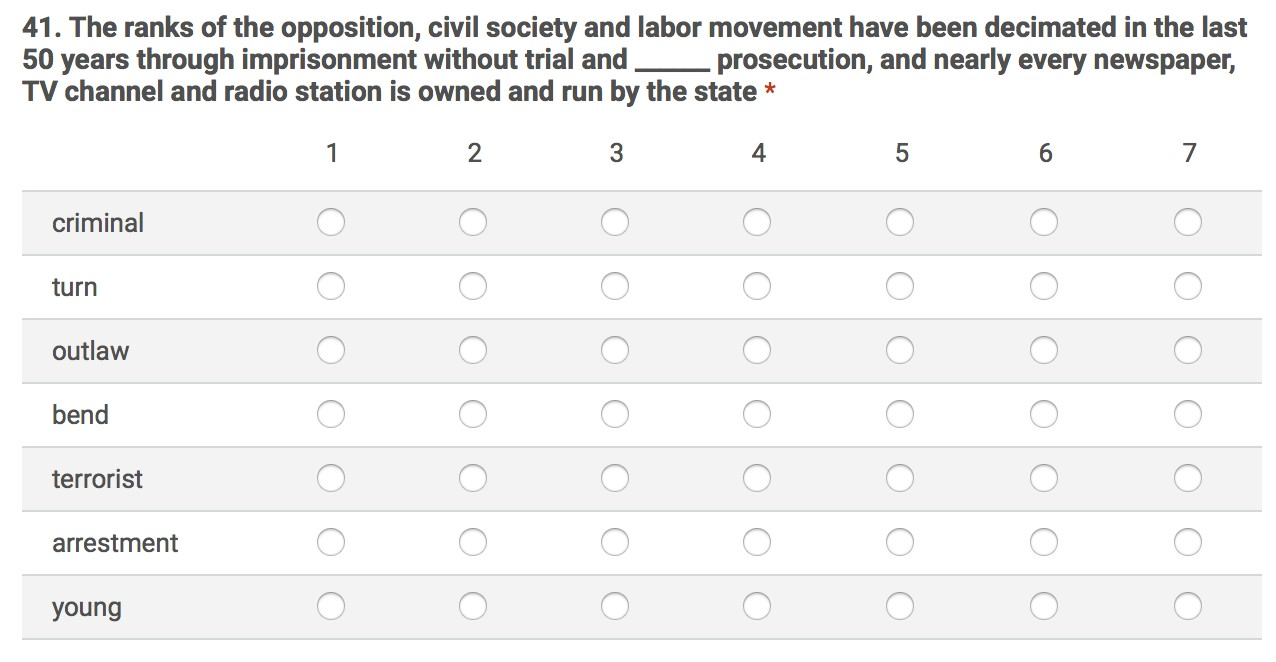
\includegraphics[width=0.45\textwidth]{distractor_1.jpg}
   \caption{A sample survey question}
   \label{fig:distractor_1}
\end{figure}
There are two evaluations to be done as follows:
1.  Compare Baseline with Knowledge Level 1 Algorithm

.  Compare Baseline with Knowledge Level 3 Algorithm
For each comparison, three distractors are generated from the baseline algorithm; three distractors are generated from the stated algorithm in this report. With the first comparison we will be able to see if the category information will help in selecting more suitable distractors. By comparing the results from the both evaluation, we will be able to see if semantic distance and category information will help improve the suitability of distractors.

\subsubsection{Results}
The evaluation contains 100 questions and is separated into 4 surveys, with each survey containing 25 questions. Each participant is free to choose one or more than one surveys. The purpose is to reduce the workload in each survey to get better responses. The surveys are sent to Year 1 students from School of Computing, National University of Singapore.  There are 15 valid responses with each participant ranking each distractor with a different weight from 1 to 7. Half of the participants are native English speakers.


Each participant’s rank will be the weight of the particular distractor in that question, i.e. if the user rank one distractor as rank “5”, the weight of this distractor in this user’s response will be 5. For each distractor of each question, the ranks of all users’ responses are summed. As the more plausible the distractor is, the higher rank it will have, thus if the sum is higher, the approach is not as plausible as the other from user’s point of view.

\begin{table}[ht]
    \caption{Comparison 1 Baseline vs. Knowledge level 1 Algorithm}
    \label{table:distractor_1}
    \begin{center}
    \begin{tabular}{| p{1.5cm} | p{2.5cm} | p{2.2cm} |}
        \hline
         & Number of winning questions & Average score\\
        \hline
        Baseline & 27 & 3.84\\
        \hline
        Level 1 Algorithm & 23 & 4.10\\
        \hline
    \end{tabular}
    \end{center}
\end{table}

\begin{table}[ht]
    \caption{Comparison 2 Baseline vs. Knowledge level 3 Algorithm}
    \label{table:distractor_2}
    \begin{center}
    \begin{tabular}{| p{1.5cm} | p{2.5cm} | p{2.2cm} |}
        \hline
         & Number of winning questions & Average score\\
        \hline
        Baseline & 21 & 4.16\\
        \hline
        Level 3 Algorithm & 29 & 3.49\\
        \hline
    \end{tabular}
    \end{center}
\end{table}

Table \ref{table:distractor_1} and Table \ref{table:distractor_2} showed the detailed result of each comparison. If for any question, the sum of weight from all participants for one approach is bigger than the other, then this approach is considered to have won this question. The “average score” is the average sum of weight from each approach for all questions. The lower the average score is, the better performance this approach has gained.

From Figure \ref{fig:distractor_1} we can see that in the first comparison, the baseline algorithm actually outscored the knowledge level 1 generation algorithm by 4 questions, with a sum of weight lower than 0.26. From Table \ref{table:distractor_1} we can see that in the second comparison, the knowledge level 3 generation algorithm surpassed the baseline algorithm by 8 questions, with the average weight of 3.49 vs 4.16. 

\subsubsection{Analysis}
In knowledge level 1 generation algorithm, there is no semantic distance calculation involved. If the target word to test has no strong category indication, for example, words like “venue”, “week”, it is possible that the knowledge level 1 algorithm will select some distractors that are not as plausible as those coming from the target word’s synonym of synonym. 

However, this problem is solved with the help of semantic distance calculator. In the knowledge level 3 generation algorithm, the distractors chosen are both semantic close and also category-related, which produced a relatively better experiment result.

Also in the baseline algorithm, it is possible that it will select words that are very rare in real life \cite{sus13}, which may also have influence in the result.

\subsection{WSD System}
Our Word Sense Disambiguate System can be evaluated from two important aspects: coverage (i.e., is able to return a translation) and accuracy (i.e., the translation is proper). To this end, I manually annotate the ground truth. Each approach was evaluated  right after I had implemented it, therefore,  they was tested against a random but different set of recent news articles from CNN.  Though the evaluation datasets are different, it is still fair to compare their results, as the size of all dataset is sufficiently large. 

Firstly, we want our algorithm to return at least one result instead of blank. For POSTagger approach, if our dictionary do not cover the Part-of-Speech generated from Stanford POSTagger, the algorithm will return nothing. For News Category approach, as the algorithm will only assign categories for some of the Chinese translations and not all Chinese news categories can match with a English news category, so the algorithm sometimes will return nothing as well. For Bing+ and Bing++ approach, if none of the Chinese translations is the substring of the Bing result, the algorithm will return nothing. For Bing++ approach, if the word alignment information is phrase to phrase matching, for example, it may give a matching between ``in order to" and its Chinese translation, the algorithm will return nothing. Alternatively, for all the listed algorithm listed above, they can always return the translation with the highest frequency of use, but in this case, we cannot know whether the result is generated from the algorithm itself or just the baseline. That's why I choose to return a blank instead of the translation with the highest frequency of use.

\begin{table}[ht]
  \caption{Coverage for different approaches}
  \label{table:evaluation_1}
  \begin{tabular}{| p{2cm} | p{2cm} | p{2cm} |}
    \hline
     & Cover & Coverage\\
    \hline
    Baseline & 707/707 & 100\%\\
    \hline
    POSTagger & 668/707 & 94.5\%\\
    \hline
    News Category & 14/707 & 2.0\%\\
    \hline
    Bing & 555/707 & 78.5\%\\
    \hline
    Bing+ & 535/707 & 75.7\%\\
    \hline
    Bing++ & 544/707 & 76.9\%\\
    \hline
  \end{tabular}
\end{table}

Table~\ref{table:evaluation_1} contains the coverage for different approaches. As the algorithm will try to translate some word only if it is covered by our dictionary, the coverage for Baseline is always 100\%. The coverage for Bing, Bing+, Bing++ and POSTagger are roughly the same and all of them are acceptable. However, the coverage for News Category approach is only 1.9\%. One reason is that when I set the threshold for assigning categories for Chinese word, I purposely make it very high to maximize the accuracy. If the accuracy is quite high, which means this approach is quite useful, then I will lower the threshold and find the balance point.
\\
Secondly, we want our algorithm to be as accurate as possible, and the most ideal situation is that all the translation returned from the algorithm is the correct or the most appropriate translation in that context. When I evaluate the accuracy of these few approaches, I use a few news articles from CNN as the input data and manually select the most appropriate translation for all the output data. After that, I will compare the result from the algorithm and the result that I manually generated and get the accuracy.

\begin{table}[ht]
  \caption{Accuracy for different approaches}
  \label{table:evaluation_3}
  \begin{tabular}{| p{2cm} | p{2cm} | p{2cm} |}
    \hline
     & Correct & Accuracy\\
    \hline
    Baseline & 405/707 & 57.3\%\\
    \hline
    POSTagger & 369/668 & 55.2\%\\
    \hline
    News Category & 1/14 & 7.1\%\\
    \hline
    Bing & 443/555 & 79.8\%\\
    \hline
    Bing+ & 433/535 & 80.9\%\\
    \hline
    Bing++ & 530/544 & 97.4\%\\
    \hline
  \end{tabular}
\end{table}

Figure~\ref{table:evaluation_3} contains the accuracy of all the approaches. The last column is the accuracy for News Category approach and it is only 30\%. As mentioned in above Chapter, since the accuracy is very low, there is no need to lower the threshold and try to allocate more categories for Chinese words. The accuracy for Baseline is 69\%, which is already a fairly hight accuracy. The accuracy for Bing and POSTagger is around 69\% also, which is a bit lower than our expectation. The accuracy for Bing++ is 97\% which I think is a very good result and it is already very hard to improve. Therefore, based on my test results, Bing++ is the best approach among these five approaches.
